\chapter{Realizace}
Aplikace je napsaná v nativním jazyku pro operační systém iOS - v Objective-C 2.0. \\Pro vývoj se používá Applem dodané IDE - Xcode a od návrhu po realizaci je třeba dodržovat pravidla společnosti Apple pro korektní vývoj aplikací. 

Aplikace napsaná nativně je nepřenositelná na jiné platformy, nicméně dosahuje nejvyšší kvality. Jsou způsoby vývoje, které zaručují přenositelný kód (HTML5 a JavaScript), většinou se ale jedná o nadstavbu nad operační systém - spustí se lokální webový server, \\a aplikace pak běží jako webová stránka. Tato možnost nepřipadala v úvahu kvůli důrazu \\na rychlost kódu a velice omezených možnostech (technologie WebSocket nedovoluje operace na nižších úrovních právě kvůli prostředí v kterém běží - localhost \cite{TIWS}) při realizaci TCP \\a UDP socketů - nejrozšířenější platforma pro vývoj aplikací pomocí JS, Phonegap, nabízí pouze WebSockety, a ty by zdaleka nevyhovovaly představám implementace.

\section{IDE}
Součástí SDK je Xcode IDE, prostředí pro efektivní vývoj aplikací. Narozdíl od jiných IDE má Xcode integrované lldb pro živé debugovaní kódu s podporou hotfixů. Živý debug spočívá v tom, že na místě, kde je nastaven breakpoint, se kód během provádění pozastaví a objeví se konzole. V konzoli je možné provádět s objekty různé základní operace - prozkoumat ukazatele a hodnoty, podívat se do paměti apod. Zároveň je z těchto poznatků možné použít právě hotfix - úpravu kódu za běhu aplikace. Lze tedy po přerušení pozastaveného kódu navázat na kód, který tam předtím nebyl.

\section{Objective-C}
Jazyk Objective-C je, jak již plyne z názvu, objektově orientovaný jazyk, který vznikl spojením jazyků C a Smalltalk. Narozdíl od jazyků podobných jazyku C používá unikátní syntaxi použitím hranatých závorek:

\begin{lstlisting}
NSString *answer = [NSString stringWithFormat:@"%d", 42];
\end{lstlisting}

Tento příkaz vytvoří nový ukazatel na objekt obsahující číslo 42, uložené jako NSString\footnote{Když chceme objekt typu NSString, musíme před uvozovky uvést znak @. Jinak se vytvoří string v jazyce C.\cite{OBJC}}. Metoda \emph{stringWithFormat:} je statická metoda objektu NSString.

Ne každý zřejmě ví, proč jsou základní objekty pojmenovány s předponou NS. V biografii Stevea Jobse \cite{STEVE} je zmíněno, že se jedná o odkaz na společnost NeXTSTEP, kterou Jobs založil po vyhazovu z Applu v roce 1985. NeXTSTEP vyvinula operační systém, který byl později koupen Applem po návratu Jobse do vedení a implementován do operačního systému Mac OS. Proto jsou základní objekty vedeny v knihovně s předponou NS \cite{NeXTSTEP}.

\section{Architektura}
Pravidla společnosti Apple směřují vývojáře, aby používali architekturu MVC při psaní aplikací. Narozdíl od Javy nefiguruje v Cocoa API explicitní balíčkovací systém, který by logicky jednotlivé vrstvy odděloval. Uživatel si může napsat vlastní framework, a pak jej zkompilovat, čímž prakticky vytvoří balíček, ale za normálních okolností se třídy do balíčků neřadí.

\subsection*{View}
Xcode IDE fyzicky odděluje grafické rozhraní v tzv. Storybardu. Jedná se o agregaci všech obrazovek a jejich návazností - scénář. Každou jednotlivou obrazovku je možné přiblížit a editovat její prvky. Editace probíhá buď intuitivním systémem drag-and-drop, nebo v XML editoru. Oba způsoby jsou vhodné pro statické navržení rozhraní, veškeré animace a pokročilé prvky je třeba realizovat v kódu controlleru, tedy nativně v Objective-C.

\subsection*{Model}
Pokud je model triviální, dovolí Xcode použití vnořené třídy, a tak celkové splynutí Controlleru a Modelu. Pokud je ale potřeba použít databázi, např. SQLite, Xcode IDE opět striktně fyzicky odděluje tuto část a zajišťuje, že si je uživatel stále vědom nutnosti držet se MVC.

\subsection*{Controller}
Veškeré třídy, které se starají o operace s daty a jejich zobrazení, musí dědit od třídy UIViewController, která má již připravené metody pro odchytávání různých eventů(scéna právě byla zobrazena nebo právě bude překryta apod.) a tím pádem je opět vývojář pobízen dodržovat MVC.

\newpage

\section{Použité klíčové knihovny}

\subsection{Core Location}
Knihovna Core Location se nachází ve druhé vrstvě operačního systému iOS - Core Services. Zabaluje informace o pozici telefonu z veškerých zdrojů, které jsou k dispozici (BTS, GPS, GLONASS a WiFi).

\subsection{Core Telephony}
Knihovna Core Telephony se roněž nachází ve druhé vrstvě operačního systému iOS - Core Services. Nabízí prostředky pro zjištění informací o domácím operátorovi sim karty v zařízení. Tato knihovna slouží primárně pro operátory, aby mohli vyvinout aplikace pouze pro vlastní zákazníky nebo pro poskytovatele VoIP, jako je Viber nebo Skype.

V implementaci je použita knihovna Core Telephony pro identifikaci operátora, jehož síť chceme změřit.

\subsection{Core Data}
Knihovna Core Data se rovněž nachází ve druhé vrstvě operačního systému iOS - Core Services. Jedná se o převodník objektů do relační databáze (ORM - Objektově relační mapování) zabalující SQLite. V implementaci aplikace slouží jako databáze, do které se ukládají vstupní a výstupní parametry každého měření. Historie se ukládá do určitého data, aby si mohl uživatel prohlížet výsledky v offline režimu (kompletní historii si může každý uživatel prohlédnout pod svým účtem na webu projektu).

Dokumentace knihovny doporučuje dotazovat databázi objektově, nikoliv SQL dotazy (lze je také použít). Při složitějších příkazech je kvalita vygenerovaných příkazů diskutabilní, nicméně filtrování řádků v aplikaci je na základní úrovni a není třeba žádných složitých SQL příkazů.

Do databáze se ukládájí veškerá sebraná a naměřená data. V průběhu měření se nesbírají souběžně informace o uživatelově pozici, pouze při zahájení a po ukončení měření. Tím pádem má aplikace k dispozici dva body, mezi kterými může vygenerovat prostor, kde probíhalo měření.

\newpage

Databáze obsahuje jednu tabulku, jelikož se ukládájí všechny parametry do jednoho řádku:

\begin{table}[h]
	\begin{center}
		\begin{tabular}{|l|l|}
			\hline
				{\bf Název} & {\bf Datový typ}\\
			\hline \hline
				Timestamp & Integer 32\\
				\hline
				StartLatitude & Double\\
				\hline
				StartLongitude & Double\\
				\hline
				StopLatitude & Double\\
				\hline
				StopLongitude & Double\\
				\hline
				Download speed & Double\\
				\hline
				Upload speed & Double\\
				\hline
				Datagram Loss & Integer 16\\
				\hline
				Average Ping & Double\\
				\hline
				Max Ping & Double\\
				\hline
				Min Ping & Double\\
				\hline
				Jitter & Double\\
				\hline
				Average Round-trip Delay Time & Double\\
				\hline
				Max Round-trip Delay Time & Double\\
				\hline
				Min Round-trip Delay Time & Double\\
				\hline
				Status Code & Integer 16\\
				\hline
		\end{tabular}
	\end{center}
	\caption{Tabulka popisující zápis v databázi}
	\label{tab.database}
\end{table}

\subsubsection*{Velikost databáze}
Data se ukládají do samostatného souboru \emph{MBTest\_model.sqlite} v rámci sandboxu aplikace. Soubor má po vytvoření před vložením dat 20kB. 

Provedl jsem test velikosti souboru při větším počtu záznamů - zvolil jsem stropní hranici testu na 200000 záznamů. Tolik záznamů uživatel posbírá za 3 týdny při periodickém měření každých 10 vteřin. Pokud bude měřit každou minutu, zvýší se čas sběru na 19 týdnů, a pokud bude měřit dvakrát za hodinu, dosáhne této hodnoty za 12 let. Test probíhal na zařízení iPhone 5 a trval 15 minut a 6 sekund. Výsledná velikost souboru byla 21,7 MB, což je v měřítku kapacity zařízení s iOS zanedbatelné číslo.

Pohled z druhé strany je takový - průměrný uživatel zařízení s iOS si po dvou letech koupí nový. Aby za dva roky naplnil databázi na danou velikost, musel by nepřetržitě měřit každých pět minut. Z toho usuzuji, že nemusím optimalizaci velikosti databáze a jejího mazání věnovat příliš pozornosti.

\newpage

\subsection{UIKit}
Knihovna UIKit se nachází ve čtvrté vrstvě operačního systému iOS - Cocoa Touch Layer. Jedná se o bohatou knihovnu pro realizaci uživatelského rozhraní. Poskytuje základní grafické ovládací prvky, ale i funkce pro odchytávání událostí, vykreslování apod. potřebné v realizaci rozhraní pro dotykovou obrazovku.

V implementaci jsou použité standardy společnosti Apple, které je třeba dodržovat při vyvíjení uživatelského rozhraní. K tomu patří například neodmyslitelný navigation bar kvůli absenci hardwarového tlačítka zpět.

\section{Externí knihovny} 
Od verze iOS 5 byla do kompilátoru implementována funkce \\{\bf Automatic Reference Counting} \cite{ARC}, která slouží ke stejnému účelu jako Garbage Collector v Javě. Rozdíl je ten, že počítá reference, a tudíž, je-li nějaký ukazatel slabý (jedná se tedy o mělkou kopii), je okamžitě uvolněn, pokud není používán. Hlavní rozdíl je tedy v tom, že uvolnění paměti neprobíhá jednou za určitou periodu, nebo pokud dojde pamět, ale vždy, když je to možné.

Tato funkcionalita výrazně zkrátila kód, neboť bez ní bylo nutné dodat, že proměnné, které jsou pouze ve scopu metody, by měly být uvolněné po doběhnutí (po každé alokované proměnné musela být uvolněna paměť). Komplikace nastala, když kompilátor pro novou verzi iOS nejenom že řádek s autorelease nepotřeboval, on dokonce vylučoval jeho přítomnost. Tato restrikce se bohužel stala překážkou v používání externích frameworků psaných pro verzy iOS 4. Kompilátor ale funguje na relativně vysoké úrovni a nabízí v Build Phases nastavení příznaku -fno-objc-arc, které vypne pro hlavičkové soubory Automatic Reference Counting, když probíhá build kódu.

\subsection{JSONKit}
Tato knihovna byla napsána pro iOS 3, a tudíž bylo nutné přidat kompilátoru příznak \\pro vypnutí ARC. Do verze iOS 5 nebyla ze strany společnosti Apple žádná nativní podpora formátu serializace JSON. Od verze iOS 5 nějaká je, ale stále nedosahuje kvalit JSONKit knihovny. V realizaci jsem ji použil pro zabalení pole do formátu JSON před odesláním pomocí HTTP POST a pro parsování přijatých dat.

Parsování probíhá zavoláním jedné metody, kterou rozšiřuje framework objekt typu NSString. Metoda z JSON stringu vytvoří objekt NSDictionary, který se chová jako standartní mapa (key, value).

\begin{lstlisting}
NSDictionary *requestDictionary = [[request responseString] objectFromJSONString];
\end{lstlisting}

Vytvoření JSON objetu probíhá obdobně, protože framework stejně rozšiřuje objekt \\NSDictionary, díky čemuž umí vytvořit JSON string z mapy.

\begin{lstlisting}
NSString *jsonData = [[NSString alloc] initWithData:dictionary encoding:NSUTF8StringEncoding];
\end{lstlisting}

\subsection{ASIHTTPRequest}
Tato knihovna byla taktéž napsána pro iOS 3 a bylo nutné opět přidat kompilátoru příznak pro vypnutí ARC. V architektuře operačního systému se nachází na úrovni Core Services. Jedná se o dlouhodobý standard mezi knihovnami, protože ASIHTTPRequest byla první knihovnou využívající asynchronní volání REST-ful operací GET / POST / PUT / DELETE.

Během realizace jsem použil metodu POST pro autorizaci uživatele, zahájení měření, nahlášení neúspěšného pokusu o měření a nahrání naměřených výsledků do databáze.

\subsubsection*{AFNetworking}
Během realizace jsem narazil na nový framework řešící RESTful architekturu. Podporuje iOS od verze 5 a novější, tudíž respektuje ARC. Workflow tohoto frameworku je ovšem velice odlišná od ASIHTTPRequest a bylo by třeba přepracovat základní stavební kameny aplikace. Zároveň autoři velmi často commitují kód na GitHub a já si nemohl dovolit používat na klíčovou část aplikace nehotový a zabugovaný framework. Pevně však věřím, že budoucnost patří AFNetworking, protože autor ASIHTTPRequest oznámil konec vývoje frameworku.

\subsection{CocoaAsyncSocket}
Tato knihovna je relativně nová, již s podporou ARC. V architektuře operačního systému se nachází na úrovni Core Services. Jedná se o lightweight knihovnu podporující TCP a UDP komunikaci. V realizaci jsem ji použil pro komunikaci se serverem (stažení a odeslání souboru za účelem změření parametrů sítě).

\subsubsection*{Technika měření}
Měření provádí server za účelem vyloučení podvodů ze strany klienta. Po zavolání metody \emph{clientHello()} obdrží klient odpověď s údaji o TCP, UDP a PING serverech. Nejprve se provede TCP měření, které probíhá následně:

\begin{enumerate}
\item {\bf SERVER:} PROTOCOL [verze]
\\ {\bf KLIENT:} SESSION [ID]
\item {\bf SERVER:} SESSION OK
\\ {\bf KLIENT:} DOWNLOAD [velikost]
\item {\bf SERVER:} [data]
\\ {\bf KLIENT:} UPLOAD [velikost]
\item {\bf SERVER:} UPLOAD GO
\\ {\bf KLIENT:} [data]
\item {\bf SERVER:} UPLOAD OK
\\ {\bf KLIENT:} QUIT
\item {\bf SERVER:} BYE
\end{enumerate}
V průběhu měření může samozřejmě nastat chyba. Pokud chyba nastane \uv{vědomě} na straně klienta, klient po selhání měření nahlásí metodou \emph{report()} backendu informace o chybě. Pokud nastane chyba, kterou odchytí server, odpoví chybovou hláškou, kterou klient zpracuje.

\begin{table}[h]
	\begin{center}
		\begin{tabular}{|l|l|}
			\hline
				{\bf Kód} & {\bf Popis}\\
			\hline \hline
				5 & Interní chyba databáze\\
				\hline
				10 & Neplatné ID sezení\\
				\hline
				11 & ID sezení je přiřazeno k jiné IP adrese\\
				\hline
				12 & Platnost ID sezení vypršela\\
				\hline
				20 & Test stahování nelze opakovat\\
				\hline
				21 & Test odesílání nelze opakovat\\
				\hline
				25 & Neplatná velikost vzorku stahování\\
				\hline
				26 & Neplatná velikost vzorku odesílání\\
				\hline
				50 & Příliš mnoho dat\\
				\hline
				51 & Neplatné ukončení dat\\
				\hline
				100 & Neplatný příkaz\\
				\hline
				101 & Neplatné ukončení příkazu (chybí CRLF)\\
				\hline
				102 & Neplatný příkaz (příliš krátký)\\
				\hline
				103 & Neplatný příkaz (příliš dlouhý)\\
				\hline
				110 & Byl očekáván příkaz SESSION\\
				\hline
		\end{tabular}
	\end{center}
	\caption{Tabulka možných chyb v průběhu TCP měření}
	\label{tab.tcp}
\end{table}

Po dokončení TCP probíhá následně UDP měření:

\begin{enumerate}
\item {\bf KLIENT:} MBTEST
\\ {\bf SERVER:} PROTOCOL [verze]
\item {\bf KLIENT:} SESSION [ID]
\\ {\bf SERVER:} START
\item {\bf KLIENT:} START
\\ {\bf SERVER:} [data]
\item {\bf KLIENT:} [data]
\\ {\bf SERVER:} QUIT
\item {\bf KLIENT:} QUIT
\\ {\bf SERVER:} BYE
\end{enumerate}

\newpage

Během komunikace může nastat chyba i zde. Na pozadí procesu běží nezávislé vlákno, které měří, jak dlouho trvá, dokud server neodpoví. Pokud neodpovídá déle jak 4 vteřiny, odešle poslední příkaz znovu. Pokud vlákno opakuje některý příkaz více jak třikrát, považuje měření za chybné a přeruší komunikaci. Pokud chybu detekuje server, opět dá vědět klientovi chybovou hláškou a klient ji zpracuje.

\begin{table}[h]
	\begin{center}
		\begin{tabular}{|l|l|}
			\hline
				{\bf Kód} & {\bf Popis}\\
			\hline \hline
				5 & Interní chyba databáze\\
				\hline
				10 & Neplatné ID sezení\\
				\hline
				11 & ID sezení je přiřazeno k jiné IP adrese\\
				\hline
				12 & Platnost ID sezení vypršela\\
				\hline
				13 & Chybný formát ID sezení\\
				\hline
				110 & Byl očekáván příkaz SESSION\\
				\hline
		\end{tabular}
	\end{center}
	\caption{Tabulka možných chyb v průběhu UDP měření}
	\label{tab.udp}
\end{table}

\begin{figure}[h]
	\centering
    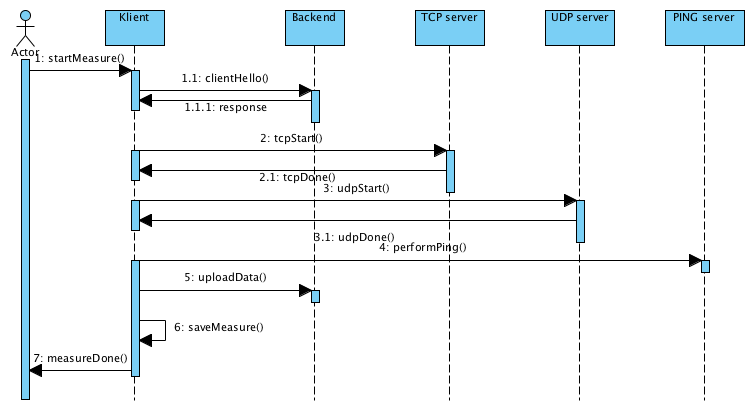
\includegraphics[width=0.8\textwidth]{figures/03_implementation/seq_diagram.jpg}
    \caption{Kompletní průběh měření}
    \label{err1}
\end{figure}

Nakonec proběhne měření odezvy proti PING serveru a spočítání hodnoty jitter. Jitter je změna velikosti zpoždění paketů a počítá se následně \cite{RFC}:

$$ J_i = \frac{J_{i-1} + (|D_{i-1,i}| - J_{i-1})}{16} $$

Výpočet jitteru probíhá iterativně. Hodnota $D_{i-1,i}$ reprezentuje vzdálenost packetů a je ekvivalentní rozdílu relativních přenosových časů. Dělení 16 probíhá pro kvalitní odstranění šumu při zachování přiměřené míry konvergence \cite{JIT}.

Tím měření končí a klient odesílá naměřené údaje na backend.

\section{Běh aplikace na pozadí}
Vyřešit běh na pozadí bylo největším oříškem celé implementace a zároveň klíčovou funkcionalitou, bez které by aplikace byla velice omezená. Základní filosofie společnosti Apple je, jak již bylo zmíněno, že aplikace bude na pozadí provádět jednu z povolených aktivit. Zároveň, jelikož se Apple snaží o to, doručit svým zákazníkům vždy špičkový software, požaduje totéž od vývojářů, a pro účely běhu na pozadí vydal rozhraní pro konkrétní implementaci. V praxi to vypadá tak, že vývojář stanoví v nastavení, že se jedná o aplikaci využívající uživatelovu polohu. Pakliže chce vývojář, aby aplikace běžela na pozadí, využije rozhraní, které odchytává \emph{změny polohy} - nikoliv v čase, nýbrž v prostoru. To bylo ale v rozporu s požadavkem na periodické měření v zadaném intervalu. 

Pokusil jsem se nejprve tuto variantu naimplementovat, tak, že jsem nastavil, aby měl \uv{locationManager}\footnote{Objekt odchytávající údaje o pozici} nejvyšší citlivost. V momentě, kdy tento objekt zachytil změnu, zkontroloval jsem čas a porovnal, jestli už uplynul dostatek od posledního měření. Poté jsem provedl měření. Tato metoda byla při standartním pohybu člověka v průběhu dne relativně přesná, nicméně v noci, kdy telefon leží na stolku, absolutně nefunkční.

Druhý způsob, který se naskytnul, bylo \uv{šťouchnutí} od serveru. Implementace spočívá \\v tom, že aplikace vyžádá ke svému certifikátu tzv. \emph{token}, který se naváže na Apple ID uživatele a zaregistruje se na Apple Push Serverech. Tento token si zároveň uloží server, z kterého bude posílána zpráva do iOS zařízení. Komunikace následně probíhá tak, že server pošle požadavek na Apple Push Server a ten to přepošle do daného iOS zařízení. Tato služba se nazývá APN (Apple Push Notification). Její implementace je elegantní v tom, že zařízení má otevřený jeden socket, přes který může přicházet velké množství zpráv. Nedrží si tak otevřené spojení s každou aplikací, a tím se šetří výdrž baterie. Tuto implementaci jsme ovšem zamítli pro vysokou časovou náročnost jak pro klienta, tak pro serverovou část. Zároveň by byla tato implementace pouze pro klienta iOS, neboť Google má pro svou platformu vlastní službu - GCM (Google Cloud Message) - a ta má zcela odlišnou implementaci.

Třetí způsob, který se nakonec ukázal jako nejefektivnější, se na první pohled zdá jako porušování pravidel Apple. Pokud má aplikace nastaveno, že podporuje běh na pozadí, pak v momentě, kdy ji uživatel minimalizuje, má 10 minut běhu, a pak se sama ukončí. Zjistil jsem, že v těchto deseti minutách stačí alespoň jednou zavolat objekt locationManager a zapnout/vypnout na něm odchytávání pozice uživatele. Tímto se prodlouží životnost probíhané aktivity o dalších 10 minut. Zajistil jsem tedy, že jednou za 9 minut (dal jsem si \\pro jistotu časový polštář) takto zařízení vyžádá pozici a běh na pozadí pokračuje.

\section{Uživatelské rozhraní}
Uživatelské rozhraní je paradoxně to nejdůležitější na celé aplikaci. Funkcionalita je upozaděna, neboť první dojem je zde absolutně klíčový. Jelikož projekt není cílený pouze na profesionály, nýbrž je určený pro širokou veřejnost, není UX\footnote{User experience} okrajovou záležitostí. Uživateli se musí aplikace na první pohled líbit, musí ihned pochopit, k čemu slouží, a zároveň musí aplikace uživateli nabídnout své služby v co nejpřívětivější formě.

Proces návrhu rozhraní podléhal následujícím kritériím:

\begin{enumerate}
	\item Co chceme uživateli prezentovat?
	\item Co všechno opravdu uživatel potřebuje vidět?
\end{enumerate}

\subsection{Pravidla Apple}
Apple si nepřeje, aby UX byla pro každou aplikaci odlišná. Chce, aby uživatelé rozuměli aplikacím hned, protože to poslední, co chce, je, aby o nich někdo říkal, že mají složitá a komplikovaná uživatelská rozhraní. Pro tyto účely vydal pokyny, jak postupovat při procesu návrhu \cite{HIG}.

\subsubsection*{UINavigationController}
Prvním základním stavebním prvkem je Navigation Controller. V hierarchii objektů je postaven nad všemi objekty typu \emph{View}. Zajišťuje přechod obrazovek, a navíc od šesté verze operačního systému iOS odchytává rotaci zařízení.

Jelikož žádný iPhone ani iPad nemají tlačítko zpět, je Navigation Controller obligátním prvkem při postupném zanořování. Uživatelé tedy vědí, že mají hledat tlačítko zpět vždy \\v horním levém rohu.

\subsubsection*{UITableView}
Apple má velice konkrétní představu o tom, jak by měly vypadat tabulky (seznamy). Uživatelé si zvykli na určité typy ikon, které naznačují, co buňka udělá, pokud ji uživatel vybere. Pokud má buňka šipku, uživatel ví, že se po vybrání zanoří hlouběji. Pokud nemá, zůstane na stejné úrovni. 

Velice zajímavý fakt je, že Apple dokázal úspěšně odstranit ze svých uživatelských rozhraní checkboxy pro seznamy. Pokud umožní programátor uživateli provést hromadnou akci s daty, učiní tak přes hromadnou selekci, která se zobrazí po stisku speciálního tlačítka.

\newpage

\subsection{Návrh}
Při navrhování jsem používal prototypovací nástroj Balsamiq, abych si vizualizoval myšlenky a zobrazení dat. Jedná se o jednoduchý WYSIWYG\footnote{What you see is what you get} editor, ve kterém můžeme rychle vytvořit uživatelské rozhraní bez dlouhého programování.

\begin{figure}[h]
	\centering
    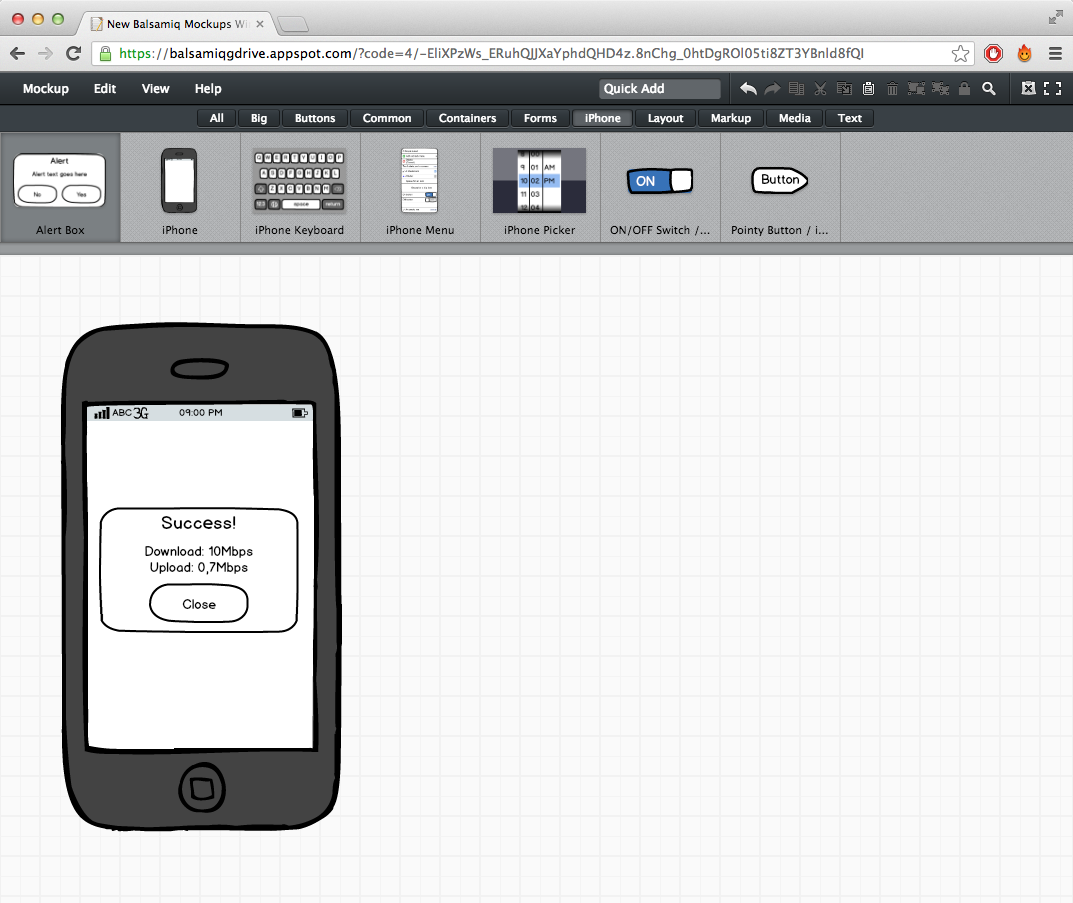
\includegraphics[width=0.8\textwidth]{figures/03_implementation/balsamiq.jpg}
    \caption{Prostředí prototypovacího nástroje Balsamiq v prohlížeči Google Chrome}
    \label{bals}
\end{figure}

\subsection*{Hlavní obrazovka aplikace}

\subsubsection*{Tab bar}
První nápad byl použít tab bar. Je univerzální, je to další ze základních stavebních prvků podle Applu a už jsem ho použil v předchozích aplikacích. Problém s tab barem je, že zůstává neustále na očích, i když ho vlastně uživatel nepotřebuje. 

{\bf Příklad:}
Uživatel začne měřit a sleduje průběh měření. Stěží ho bude zajímat kompletní historie měření. Buď měří jednorázově, tudíž se mu zobrazí výsledek po dokončení měření, nebo měří periodicky a zajímají ho dílčí výsledky provedené v probíhajícím sezení. V tomto případě je spodní bar k ničemu, protože nelze nastavit, aby se choval dvojím způsobem - jeho chování bude vždy konstantní.

Zároveň tab bar určuje jakousi paralelní souběžnost akcí pod jednotlivými záložkami, což je nesmysl, neboť během měření by nemělo být umožněno uživateli měnit nastavení svého účtu. Z toho jsem usoudil, že tab bar není vhodným středobodem rozhraní.

\subsubsection*{Dashboard}
Vrátil jsem se zpět k požadavkům a snažil si uspořádat myšlenky pro nejvhodnější rozložení aplikace. Dospěl jsem k názoru, že dashboard bude optimálním řešením. Nebudu mást uživatele výběrem více obrazovek v tab baru. Po přihlášení dostane na výběr:

\begin{enumerate}
	\item Prohlížet výsledky
	\item Měřit
\end{enumerate}

Pokud si bude chtít prohlédnout dílčí výsledky během měření, podívá se přímo z měření přes speciální tlačítko. Nebude tak muset zkoumat, které výsledky byly v daném měření naměřeny, protože dotaz do databáze se bude vztahovat pouze k danému průběhu.

\subsection*{Zobrazení výsledků}
Výsledky lze zobrazit v seřazeném seznamu podle času měření. Seznam je oddělován delimitery po jednotlivých dnech. Zajímavostí seznamu je, že se dynamicky překreslí, pokud je do databáze zapsáno nové měření. K realizaci takového dynamického seznamu je určeno rozhraní \emph{NSFetchedResultsControllerDelegate} z frameworku Core Data. Pro plnou funkčnost je třeba implementovat čtyři metody:

\begin{enumerate}
	\item
	\emph{- (void)controllerWillChangeContent:(NSFetchedResultsController *)controller}
	
	Zde se musí zavolat metoda \emph{beginUpdates} na objektu \emph{UITableView}, díky kterému se tabulka zamkne a je možné ji bezpečně\footnote{thread safe} začít aktualizovat.
	
	\item
	\emph{- (void)controller:(NSFetchedResultsController *)controller didChangeSection:\\(id <NSFetchedResultsSectionInfo>)sectionInfo atIndex:(NSUInteger)sectionIndex \\forChangeType:(NSFetchedResultsChangeType)type}
	
	Tato metoda se stará o konzistenci jednotlivých sekcí. Jak je zmíněno výše, sekce jsou děleny po jednotlivých dnech.
	
	\item
	\emph{- (void)controller:(NSFetchedResultsController *)controller didChangeObject:\\(id)anObject atIndexPath:(NSIndexPath *)indexPath forChangeType:\\(NSFetchedResultsChangeType)type newIndexPath:(NSIndexPath *)newIndexPath}
	
	Tato metoda je k dispozici pro odlišení, zda byl objekt z databáze smazán, nebo byl nový objekt přidán. Slouží pro identifikaci nové akce a zapracování animace.

	\item
	\emph{- (void)controllerDidChangeContent:(NSFetchedResultsController *)controller}
	
	Pokud je tato metoda zavolána, znamená to, že veškeré úpravy byly dokončeny. Programátor by v této metodě měl uvolnit paměť, kterou použil při aktualizaci tabulky, a nakonec by ji měl odemknout. Tím proces končí.
\end{enumerate}

\subsection{Grafické zpracování}
Pro zpracování grafického vzhledu rozhraní jsem použil Adobe Photoshop CS 5.5. V průběhu implementace jsem našel v designu zalíbení, nicméně časová náročnost byla velmi vysoká, protože jsem neznal prostředí Photoshopu, a celý týden jsem se snažil zorientovat ve všech funkcionalitách.

\subsubsection*{Barvy a logo}
Během diskuzí s celým týmem došlo ke sjednocenému názoru, že aplikace by měla být laděná do tónů modré barvy. Osobně preferuji realistické barvy nad pastelové, rozhodl jsem se tedy podtrhnout barvy světlem a logo jsem vytvořil stříbrné. Obě zmíněné konkurenční aplikace mají v logu tachometr, proto jsem tvorbu loga odlišil. Nebyl jsem si jistý, co použít a chtěl jsem se vyhnout klišé tachometru. Prozatím zůstává tedy logem stříbrný nápis MBTest \\s použitým písmem Agency FB. Výsledné logo a postup jeho přípravy se nachází v příloze.

\subsubsection*{Rozměry obrazovek}
Do vydání páté generace iPhone měl Apple velice chytře vyřešenou otázku rozlišení. Všechny modely do verze 3GS měly stejné displaye. První verze s displayem \emph{retina}, iPhone 4, předchozí rozlišení zdvojnásobil, tudíž byly zachované poměry stran. V praxi to fungovalo následovně:

Jedno tlačítko má rozměr 30 x 80 na nižším rozlišení a 60 x 160 na vyšším. Projekt tedy musí obsahovat dva PNG soubory - btn\_img.png a btn\_img@2x.png. Klíčové rozšíření je \uv{@2x}, které dává kompilátoru pokyn pro výběr tohoto souboru pro vytvoření GUI pro iPhone s vyšším rozlišením.

\begin{table}[h]
	\begin{center}
		\begin{tabular}{|l|l|}
			\hline
				{\bf Model} & {\bf Rozlišení}\\
			\hline \hline
				iPhone & 320 x 480\\
				\hline
				iPhone 3G & 320 x 480\\
				\hline
				iPhone 3GS & 320 x 480\\
				\hline
				iPhone 4 & 640 x 960\\
				\hline
				iPhone 4S & 640 x 960\\
				\hline
				iPhone 5 & 640 x 1136\\
				\hline
		\end{tabular}
	\end{center}
	\caption{Tabulka rozlišení jednotlivých modelů iPhone}
	\label{tab.resphone}
\end{table}

Jak je patrné z tabulky, model iPhone 5 má odlišný poměr stran od ostatních modelů a vyladění drobných detailů v grafickém rozhraní se musí řešit v kódu, čímž kód poněkud klesá na kvalitě a přenosnosti.

\newpage
Tablety iPad jsou v tomto ohledu jednotné a veškeré modely si zachovaly stejný poměr stran.

\begin{table}[h]
	\begin{center}
		\begin{tabular}{|l|l|}
			\hline
				{\bf Model} & {\bf Rozlišení}\\
			\hline \hline
				iPad & 1024 x 768\\
				\hline
				iPad 2 & 1024 x 768\\
				\hline
				iPad 3 & 2048 x 1536\\
				\hline
				iPad 4 & 2048 x 1536\\
				\hline
				iPad mini & 1024 x 768\\
				\hline
		\end{tabular}
	\end{center}
	\caption{Tabulka rozlišení jednotlivých modelů iPad}
	\label{tab.restab}
\end{table}

Nasazení grafiky u iPadu pro vyšší rozlišení funguje stejně jako u iPhone. Na konferenci společnosti Apple - WWDC 2013 mají být odhaleny nové verze obou stávajících modelů tabletu iPad, nicméně indície vedou ke stejnému rozlišení u obou verzí (2048 x 1536).